	
\section{The Code}
	\section{Time evolution: Euler's method}
	\subsection{The Random Force}
\section{Determining constants of the model}
The stalk and tail lengths $\ell_S, \ell_T$ as well as a set of equilibrium angles $\{\varphi_{i,\text{eq}}\}$ were determined by examining microscopy images of dynein in various configurations. 
\begin{figure}[hbt!]
	\centering
	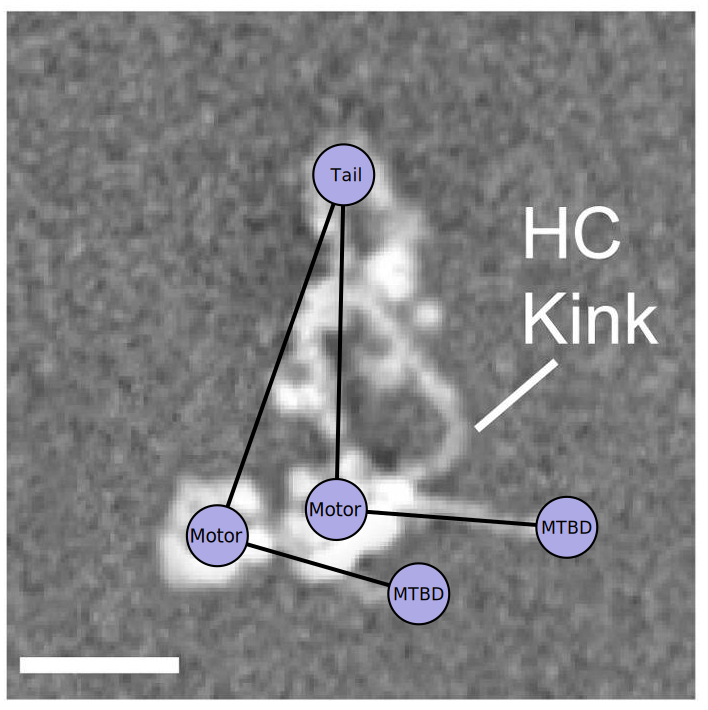
\includegraphics[width=0.3\columnwidth]{schematic-2-superimposed}
	\caption{Our model superimposed over microscopy image of Dynein \textbf{NOTE: add source} for determining lengths and equilibrium angles} 
	\label{fig:superimpmosed}
\end{figure}

\section{Testing the model} 
\subsection{Sanity Checks}
This sub section will be for the various methods we used to ensure our model is behaving reasonably 
\subsubsection{Verifying size of time step} 
Here I will talk about how we found autocorrelations functions for each domain energy at various values of dt in order to verify our time step is as large as can be
\subsubsection{Energy conservation and the Equipartion theorem} 
talk about code to check that we satisfy energy 
\subsection{Fitting to other studies} 	